\newpage
\begin{center}
  \textbf{\large 3. Построение преобразователей угол-код на синусно-косинусных решающих устройствах}
\end{center}
\refstepcounter{chapter}
\addcontentsline{toc}{chapter}{3. Построение преобразователей угол-код на синусно-косинусных решающих устройствах}


\section{Классические схемы и их эволюция}

Существует широкий класс схем посмотроенич преобразоваталей угол-код.
В литературе, \cite{Vulvet}, описаны различные методы построения преобразователей угол-код. 
Среди цифровых кодирующих преобразователей угловых перемещений существует два основных класса: 
\begin{itemize}
  \item Преобразователи абсолютных значений
  \item Накапливающие преобразователи 
\end{itemize}

\begin{itemize}
  \item Контактные кодирующие преобразователи 
  \item Магниторезистивные преобразователи
  \item Аналоговые схемы с использованием \textbf{RLC-цепей} для формирования сигналов.
  \item Трансформаторные системы, основанные на взаимной индукции.
\end{itemize}

Однако такие решения обладают некоторыми существенными недостатками в современных условиях:
\begin{itemize}
  \item \textbf{Считывание}: Использование моточных изделий (трансформаторов, катушек) увеличивает массу и габариты устройств.
  \item \textbf{Устаревание}: В связи с совершенствованием схем контроллеров, появляются возможности для более оптимальных.
  \item \textbf{Сложность настройки}: Требуется точная подстройка аналоговых компонентов, что снижает надежность.
  \item \textbf{Низкая совместимость} с цифровыми системами управления.
\end{itemize}

Развитие микропроцессорной техники и миниатюризация контроллеров привели к переходу на компактные и энергоэффективные решения. 
Современные преобразователи исключают громоздкие аналоговые компоненты, заменяя их программируемыми схемами.

\section{Современные подходы}

В контексте оптимизации веса, габаритов и точности рассматриваются два основных типа схем:

\begin{enumerate}
    \item \textbf{Цифровые преобразователи на базе микроконтроллеров}:
    \begin{itemize}
        \item Используют АЦП и алгоритмы цифровой обработки сигналов (ЦОС).
        \item Лишены моточных элементов, что снижает массу на 30–40\%.
        \item Обеспечивают точность до \(\pm0.1^\circ\) за счет программной компенсации погрешностей.
    \end{itemize}
    
    \item \textbf{Гибридные схемы с интегрированными ИС}: 
    \begin{itemize}
        \item Комбинируют аналоговые синусно-косинусные генераторы и цифровые интерфейсы (SPI, I\(^2\)C).
        \item Применяют специализированные микросхемы (например, AD2S1210), минимизирующие число внешних компонентов.
        \item Поддерживают разрешение до 16 бит при компактных размерах.
    \end{itemize}
    Например на рынке доступна микросхема К1310НМ025. \cite{Spec}
\end{enumerate}

\subsection{Преимущества современных решений}
\begin{itemize}
    \item \textbf{Миниатюризация}: Отказ от трансформаторов снижает объем устройства в 2–3 раза.
    \item \textbf{Повышенная надежность}: Цифровая обработка исключает дрейф параметров аналоговых компонентов.
    \item \textbf{Совместимость}: Интеграция с промышленными сетями (CAN, Ethernet) упрощает внедрение.
\end{itemize}

Таким образом, классические схемы, описанные в ранних работах, уступают современным цифровым и гибридным решениям по ключевым параметрам. 
Переход на микроконтроллерные системы и специализированные ИС позволяет достичь высокой точности при минимальных массогабаритных показателях, 
что особенно актуально для аэрокосмических и робототехнических применений

В части цифровой обработки сигналов дачтчиков рассматриваются две основныеы схемы

\subsection{Метод прямого преобразования}
\subsubsection{Принцип работы}
Метод прямого преобразования \cite{Armenski} основан на вычислении угла поворота через арктангенс отношения синусоидального (\(U_{\sin}\)) и косинусоидального (\(U_{\cos}\)) сигналов:
\[
\theta = \arctan\left(\frac{U_{\sin}}{U_{\cos}}\right).
\]
Для реализации метода используются два АЦП, оцифровывающих сигналы с датчика. Разрядность АЦП напрямую влияет на точность: 
\[
\Delta\theta = \frac{360^\circ}{2^N},
\]
где \(N\) — разрядность АЦП. Например, для \(N = 12\) бит:
\[
\Delta\theta = \frac{360^\circ}{4096} \approx 0.088^\circ.
\]

\subsubsection*{Пример реализации}
\begin{itemize}
    \item \textbf{АЦП}: 14-битный, частота дискретизации 100 кГц.
    \item \textbf{Алгоритм}: Коррекция нелинейностей методом таблицы поиска (LUT).
    \item \textbf{Точность}: \(\pm0.05^\circ\) при \(N=16\).
\end{itemize}
\section{Проблемы метода прямого преобразования}
Метод прямого преобразования угла в код через вычисление арктангенса отношения синусоидального и косинусоидального сигналов сталкивается со следующими ограничениями:

\subsection{Основные недостатки}
\begin{itemize}
    \item \textbf{Зависимость от качества сигналов} \\
    Шумы, нелинейности и фазовые сдвиги в сигналах \( U_{\sin} \) и \( U_{\cos} \) приводят к систематическим ошибкам. Например, асимметрия амплитуд вызывает погрешность:
    \[
    \Delta\theta = \arctan\left(\frac{U_{\sin} + \delta}{U_{\cos}}\right) - \arctan\left(\frac{U_{\sin}}{U_{\cos}}\right),
    \]
    где \(\delta\) — отклонение амплитуды.

    \item \textbf{Высокие требования к АЦП} \\
    Для точности \(\Delta\theta < 0.1^\circ\) требуется разрядность АЦП не менее 16 бит:
    \[
    N = \log_2\left(\frac{360^\circ}{\Delta\theta}\right) \approx 16.
    \]

    \item \textbf{Нелинейности и калибровка} \\
    Отклонения от идеальной синусоиды требуют использования таблиц поправок (LUT), увеличивая сложность алгоритма.

    \item \textbf{Чувствительность к внешним факторам} \\
    Температурный дрейф компонентов (например, АЦП) снижает стабильность:
    \[
    \Delta\theta_{\text{дрейф}} = \alpha \cdot \Delta T,
    \]
    где \(\alpha\) — температурный коэффициент, \(\Delta T\) — перепад температуры.

    \item \textbf{Ограниченная скорость обработки} \\
    Вычисление \(\arctan\) и коррекция занимают время \( t_{\text{проц}} \propto N \), ограничивая частоту обновления.

    \item \textbf{Проблемы при малых сигналах} \\
    При \(\theta \to 0^\circ\) или \(90^\circ\) отношение \( U_{\sin}/U_{\cos} \) стремится к \(0\) или \(\infty\), увеличивая погрешность из-за дискретизации.

    \item \textbf{Зависимость от опорного напряжения} \\
    Погрешность опорного напряжения \(\Delta V_{\text{ref}}\) вносит дополнительную ошибку:
    \[
    \Delta\theta_{\text{ref}} = \frac{\Delta V_{\text{ref}}}{V_{\text{ref}}} \cdot 360^\circ.
    \]
\end{itemize}

\subsection{Пример практического применения}
Для 12-битного АЦП теоретическая погрешность составляет:
\[
\Delta\theta = \frac{360^\circ}{2^{12}} \approx 0.088^\circ.
\]
Однако при уровне шума \(1\%\) реальная точность ухудшается до \(0.5^\circ\).

\subsection{Заключение}
Метод прямого преобразования подходит для статических систем с умеренными требованиями к точности. В динамических или высокоточных приложениях предпочтительны следящие преобразователи с обратной связью, компенсирующие перечисленные недостатки.
\textbf{Недостатки:}
\begin{itemize}
    \item Зависимость от качества сигналов (шумы, искажения).
    \item Высокие вычислительные затраты при использовании высокоразрядных АЦП.
\end{itemize}

\subsection{Следящие преобразователи}
\cite{Safronov}
\subsubsection*{Принцип работы}
Следящие преобразователи (СП) используют замкнутый контур управления для минимизации рассогласования между текущим углом и заданным значением. Сигналы \(U_{\sin}\) и \(U_{\cos}\) сравниваются с опорными, а ошибка подается на корректирующий элемент (например, двигатель).

\subsubsection*{Структура СП}
\begin{itemize}
    \item \textbf{Фазовый детектор}: Вычисляет разность фаз между входными и опорными сигналами.
    \item \textbf{Интегратор}: Формирует управляющий сигнал для исполнительного механизма.
    \item \textbf{Обратная связь}: Обеспечивает точность \(\pm0.01^\circ\) за счет коррекции в реальном времени.
\end{itemize}

\subsubsection*{Сравнение с прямым методом}
\begin{table}[ht]
    \centering
    \caption{Сравнение методов преобразования}
    \begin{tabular}{|l|c|c|}
        \hline
        \textbf{Параметр} & \textbf{Прямое преобразование} & \textbf{Следящий СП} \\ \hline
        Точность & \(\pm0.05^\circ\) & \(\pm0.01^\circ\) \\ \hline
        Быстродействие & 1 мс & 0.1 мс \\ \hline
        Сложность & Низкая & Высокая \\ \hline
        Применение & Статичные системы & Динамические системы \\ \hline
    \end{tabular}
\end{table}

\subsubsection*{Современные реализации}
\begin{itemize}
    \item \textbf{Цифровые СП на ПЛИС}: Используют алгоритмы PID-регулирования и адаптивную фильтрацию.
    \item \textbf{Пример}: СП на базе микроконтроллера STM32H7 с разрешением 18 бит и частотой обновления 10 кГц.
\end{itemize}

\subsection*{Заключение}
\begin{itemize}
    \item \textbf{Прямое преобразование} подходит для систем с умеренными требованиями к скорости и точности.
    \item \textbf{Следящие преобразователи} обеспечивают прецизионное управление в динамических системах, но требуют сложной настройки.
\end{itemize}




\section{Техническое задание на устройство}

Было принято решение о собственной разработке печатного узла на базе stm32F7.


\subsection{НАЗНАЧЕНИЕ И СОСТАВ ИЗДЕЛИЯ}

Блок аналого-цифрового преобразователя вращающегося трансформатора (далее АЦПВТ, блок АЦПВТ, изделие) предназначен для определения углового положения одной из координат антенной системы. 
Работа АЦПВТ ведется по двухотсчетной схеме с величиной редукции от датчика грубого отсчета к датчику точного отсчета 1/36.  

\textbf{ОСНОВНЫЕ ТЕХНИЧЕСКИЕ ТРЕБОВАНИЯ}

\begin{itemize}
    \item На рисунке ~\ref{FuncBlocks}, упрощенно показана структурная схема изделия. 
          С помощью разъема СНП-59 блок подключается к датчикам углового положения и концевым выключателям приборного редуктора. 
          Внутри блока расположены схемы обработки сигналов вращающихся трансформаторов и концевых выключателей. 
          Преобразованные с помощью данных схем сигналы затем отправляются с помощью микроконтроллера и приемо-передатчика ведущему устройству.  

    \item Дополнительно в изделии установлен разъем, подключенный параллельно концевым выключателям приборного редуктора с целью реализации цепей безопасности, 
          например подключение невозвратных концевых выключателей последовательно в цепь питания главного контактора шкафа электропривода. 

        \begin{figure}[!t]
          \centering
          \includegraphics[width=150mm ]{FuncBlocks.jpg} 
          \caption{Эскиз функциональных блоков изделия}
          \label{FuncBlocks}
        \end{figure}

    \item Изделие должно функционировать с вращающимися трансформаторами типа ЛИР-ДР158А.
      \end{itemize}


    В качестве интерфейса информационного обмена должен использоваться последовательный SSI со следующими параметрами:
    \begin{itemize}
          \item частота следования импульсов сигнала «Clock» 100кГц,
          \item  формирование телеграммы блока АЦПВТ должно происходить при использовании кода Грея. 
    \end{itemize}
    В телеграмме 18 бит, начиная со старшего (MSB), должны быть использованы для передачи углового положения координаты антенны. 

    На этапе программирования должна быть осуществлена стыковка с модулем подключения энкодеров SMC30 преобразователя частоты Sinamics S-120 и проверка совместного функционирования. 

\textbf{КОНСТРУКТИВНЫЕ ТРЕБОВАНИЯ}
        Конструктивно блок АЦПВТ должен представлять из себя картридж, который вставляется в корпус приборного редуктора. 
        После стыковки блока АЦПВТ и приборного редуктора обеспечивается герметичность узла. 

        Cхема блока размещена на одной печатной плате, габариты которой задаются эскизом корпуса блока АЦПВТ (см. рисунки \ref{Corp1}, \ref{Corp2}). 

        \begin{figure}[!t]
          \centering
          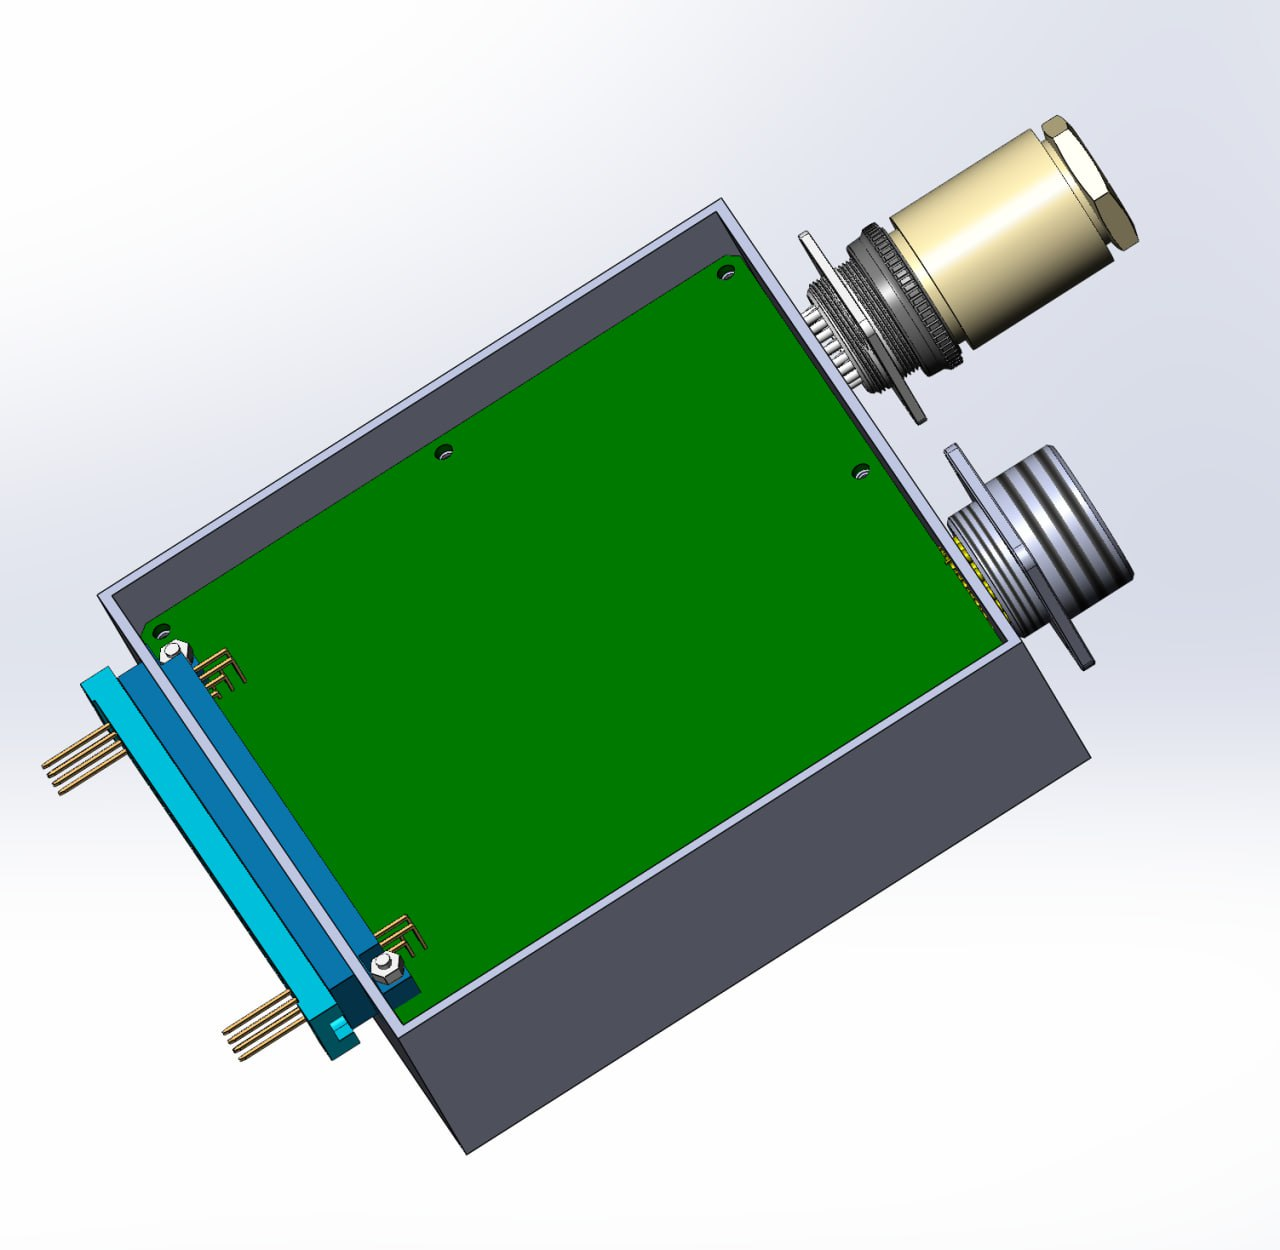
\includegraphics[width=150mm ]{Corp1.jpg} 
          \caption{Корпус блока}
          \label{Corp1}
        \end{figure}

        \begin{figure}[!t]
          \centering
          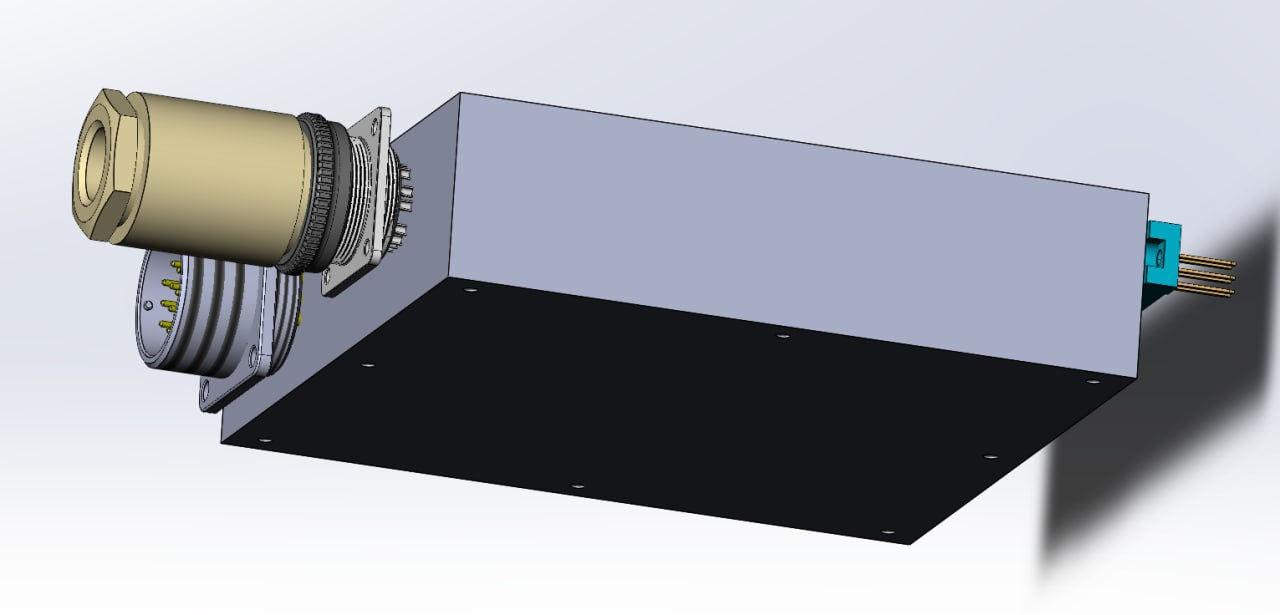
\includegraphics[width=150mm ]{Corp2.jpg} 
          \caption{Корпус блока}
          \label{Corp2}
        \end{figure}

  \textbf{ТРЕБОВАНИЯ УСТОЙЧИВОСТИ К ВНЕШНИМ ВОЗДЕЙСТВИЯМ}
  Требования по стойкости к воздействию климатических факторов:
\begin{itemize}

  \item пониженная температура рабочая – минус 40°С;

  \item пониженная температура предельная – минус 60°С;

 \item повышенная температура рабочая – плюс 60°С;

 \item повышенная температура предельная – плюс 70°С;

 \item относительная влажность – до 95 процентов при температуре плюс 30°С;

 \item иней и роса – температура минус 25°С, длительность воздействия до 2 часов;

 \item соляной туман в циклическом режиме.

\end{itemize}


\section{Узел печатный}

По итогам проведёного НИР был изготовлен узел печатный блока АЦПВТ. Для создания возбуждающего синусоидального сигнала был выбран внешний ЦАП, подключенный к целому порту. 
Для обработки сигналов двух датчиков установлены внешние АЦП, на каждый их них также выделено по целому порту для удобства использования. Для синхронизации была реализована схема 
работы аппаратных таймеров в режиме взаимодействия ведущий - ведомый. (см. рис. ~\ref{Timers})


\begin{figure}[!h]
  \centering
  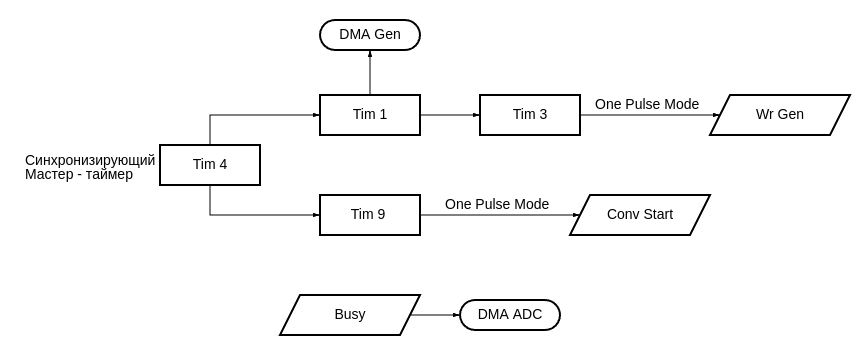
\includegraphics[width=150mm ]{TimersScheme1.png} 
  \caption{Схема взаимодействия таймеров}
  \label{Timers}
\end{figure}

Мастер-таймер 4 синхронно запускает таймеры 3 и 9. Таймер 3 запускает DMA (Direct Memory Access - переферия для доступа в память без участия процессора) на передачу нового значения в порт ЦАП.
После передачу он в режиме one-pulse-mode подает сигнал (Write Gen) на пин микросхемы, начиная загрузку значения из параллельного порта во внутренний регистр ЦАП. Таймер 9 нужен для задержки подачи
сигнала начала преобразования АЦП (Conversion start), чтобы делать выборку по амплитуде сигнала с датчика ЛИР-ДР158А, увеличивая тем самым точность расчетов.

Взятие данных с параллельного порта АЦП происходит также посредствам DMA в момент получения прерывания по спадающему фронта сигнала Busy. Так как этот сигнал через логические "ИЛИ" 
заведен на все 4 микросхемы АЦП, то значения снимаются со всех АЦП после окончания преобразования последнего. 
\textbf{схемы включения АЦП и ЦАП}

\textbf{Картинка синуса с ЦАП}

\section{Разработка следящего алгоритма}

В рамках разработки системы обработки сигналов датчиков угловых перемещений ЛИР-ДР158А был выбран метод следящего преобразования. Данный метод, 
описанный в статье \cite{Anufriev2014}, позволяет минимизировать систематические ошибки и повысить разрешающую способность преобразователя. Е
го ключевая идея заключается в использовании контура обратной связи, компенсирующего фазовые и скоростные рассогласования.

\subsection{Принцип работы следящего алгоритма}
Структурная схема следящего преобразователя представлена на схеме рис. \ref{fig:tracking_scheme}. 

\begin{figure}[ht]
  \resizebox{150mm}{!}{%
  \begin{tikzpicture}[
      block/.style={
          rectangle, 
          draw, 
          text width=6em, 
          text centered, 
          minimum height=3em, 
          font=\small,
          rounded corners=3pt
      },
      arrow/.style={->, thick, >=stealth},
      node distance=1.2cm and 0.8cm,
    ]
  
  % Блоки
  \node[block] (multSin) {Умножитель на $\sin(\phi')$};
  \node[block, below=of multSin] (multCos) {Умножитель на $\cos(\phi')$};
  \node[block, right=of multSin] (detector) {Детектор ошибки};
  \node[block, right=of detector] (integrator) {Интегратор угла};
  
  % Сигналы
  \node[left=of multSin] (inputSin) {$ V sin(\omega t) sin(\phi)$};
  \node[left=of multCos] (inputCos) {$ V sin(\omega t) cos(\phi)$};
  \node[right=of integrator] (output) {$\omega$};
  
  % Обратная связь: phi' к умножителям
  \coordinate (feedback) at ($(integrator.east)!0.5!(output.west)$);
  \node[above=0.3cm of feedback, font=\scriptsize] {};
  \draw[arrow, dashed, red] (integrator.north) -- ++(0.5cm,0) |- ([yshift=1cm]multSin.north) -- (multSin.north);
  \draw[arrow, dashed, red] (integrator.south) -- ++(0.5cm,0) |- (multCos.east); %([yshift=1cm]multCos.south) -- 
  
  % Основные соединения
  \draw[arrow] (inputSin) -- (multSin);
  \draw[arrow] (inputCos) -- (multCos);
  \draw[arrow] (multSin) -- (detector);
  \draw[arrow] (multCos) -- (detector);
  \draw[arrow] (detector) -- node[below=0.7cm] {} (integrator);
  \draw[arrow] (integrator) -- (output);
  
  % Пояснение обратной связи
  \node[above=0.1cm of multSin, align=center, font=\scriptsize] {};
  \node[below=0.1cm of multCos, align=center, font=\scriptsize] {Обратная связь: \\ $\phi'$ обновляется \\ через интегратор};
  
  \end{tikzpicture}
  } % Конец resizebox
  \caption{Схема следящего преобразователя с обратной связью.} % Красные пунктирные линии показывают передачу оценки угла $\phi'$ обратно в умножители.
  \label{fig:tracking_scheme}
  
  \end{figure}
  

Алгоритм включает следующие этапы:
\begin{enumerate}
    \item \textbf{Умножение сигналов:} Входные сигналы \( V_{\text{sin}} \) и \( V_{\text{cos}} \) умножаются на синтезированные опорные сигналы \( \sin(\phi') \) и \( \cos(\phi') \), где \( \phi' \) — текущая оценка угла. 
    \item \textbf{Детектирование ошибки:} Результирующий сигнал ошибки формируется как: 
    \begin{equation}
      e = V sin(\omega t) sin(\phi) \cdot cos(\phi') - V sin(\omega t) cos(\phi) \cdot sin(\phi') = V sin(\omega t) \cdot \sin(\phi - \phi'),
      \label{eq:error}
    \end{equation}
    % \[
    % e = V sin(\omega t) sin(\phi) \cdot cos(\phi') - V sin(\omega t) cos(\phi) \cdot sin(\phi') = V sin(\omega t) \cdot \sin(\phi - \phi') .
    % \]
    Для малых рассогласований \( \phi - \phi' \) ошибка пропорциональна разности углов ($\sin(\phi - \phi') \approx \phi - \phi'$).
    \item \textbf{Интегрирование:} Сигнал ошибки интегрируется для расчёта угловой скорости \( \omega \), а затем — угла \( \phi' \). 
    \begin{equation}
      \phi'(t) = \phi'(0) K_i \int_0^t \sin\left(\phi(\tau) - \phi'(\tau)\right) d\tau,
      \label{eq:phi_prime}
    \end{equation}
      
      где:
    \begin{itemize}
        \item \(K_i\) — коэффициент усиления интегратора,
        \item \(\phi(\tau)\) — истинный угол (измеряемый датчиком),
        \item \(\phi'(0)\) — начальное условие (оценка угла в момент \(t=0\)).
    \end{itemize}


    %Интегратор устраняет постоянную составляющую ошибки, обеспечивая нулевую погрешность при постоянной скорости вращения.
\end{enumerate}

\subsection{Преимущества и ограничения}
Метод следящего преобразования обладает следующими преимуществами:
\begin{itemize}
    \item Компенсация систематических ошибок при постоянной скорости вращения.
    \item Высокая разрешающая способность (до 19 бит для двухотсчётных систем).
    \item Фильтрация помех в контуре обратной связи, что повышает отношение сигнал/шум.
\end{itemize}

Однако алгоритм имеет ограничения:
\begin{itemize}
    \item Чувствительность к неоднородности параметров обмоток СКВТ.
    \item Ошибки при ускорении датчика, связанные с ограниченной полосой пропускания контура \cite{Anufriev2014}.
\end{itemize}

\subsection{Реализация в печатной плате}
Разработанный алгоритм интегрирует следящий алгоритм.

\section{Испытательный стенд}

Для проведения испытаний бы изготовлен стенд c двумя датчиками ЛИР-ДР158А с передаточным отношением 1/36. 
С помощью специально подготовленного переходника, блок АЦПВТ был подключен к установке. \textbf{Вставить фото подключенного стенда к АЦПВТ}
Сигналы с датчика стали поступать на АЦП \textbf{картинка кинсуов с датчика}